% Options for packages loaded elsewhere
% Options for packages loaded elsewhere
\PassOptionsToPackage{unicode}{hyperref}
\PassOptionsToPackage{hyphens}{url}
\PassOptionsToPackage{dvipsnames,svgnames,x11names}{xcolor}
%
\documentclass[
  11pt,
]{article}
\usepackage{xcolor}
\usepackage[margin=1in]{geometry}
\usepackage{amsmath,amssymb}
\setcounter{secnumdepth}{5}
\usepackage{iftex}
\ifPDFTeX
  \usepackage[T1]{fontenc}
  \usepackage[utf8]{inputenc}
  \usepackage{textcomp} % provide euro and other symbols
\else % if luatex or xetex
  \usepackage{unicode-math} % this also loads fontspec
  \defaultfontfeatures{Scale=MatchLowercase}
  \defaultfontfeatures[\rmfamily]{Ligatures=TeX,Scale=1}
\fi
\usepackage{lmodern}
\ifPDFTeX\else
  % xetex/luatex font selection
\fi
% Use upquote if available, for straight quotes in verbatim environments
\IfFileExists{upquote.sty}{\usepackage{upquote}}{}
\IfFileExists{microtype.sty}{% use microtype if available
  \usepackage[]{microtype}
  \UseMicrotypeSet[protrusion]{basicmath} % disable protrusion for tt fonts
}{}
\makeatletter
\@ifundefined{KOMAClassName}{% if non-KOMA class
  \IfFileExists{parskip.sty}{%
    \usepackage{parskip}
  }{% else
    \setlength{\parindent}{0pt}
    \setlength{\parskip}{6pt plus 2pt minus 1pt}}
}{% if KOMA class
  \KOMAoptions{parskip=half}}
\makeatother
% Make \paragraph and \subparagraph free-standing
\makeatletter
\ifx\paragraph\undefined\else
  \let\oldparagraph\paragraph
  \renewcommand{\paragraph}{
    \@ifstar
      \xxxParagraphStar
      \xxxParagraphNoStar
  }
  \newcommand{\xxxParagraphStar}[1]{\oldparagraph*{#1}\mbox{}}
  \newcommand{\xxxParagraphNoStar}[1]{\oldparagraph{#1}\mbox{}}
\fi
\ifx\subparagraph\undefined\else
  \let\oldsubparagraph\subparagraph
  \renewcommand{\subparagraph}{
    \@ifstar
      \xxxSubParagraphStar
      \xxxSubParagraphNoStar
  }
  \newcommand{\xxxSubParagraphStar}[1]{\oldsubparagraph*{#1}\mbox{}}
  \newcommand{\xxxSubParagraphNoStar}[1]{\oldsubparagraph{#1}\mbox{}}
\fi
\makeatother


\usepackage{longtable,booktabs,array}
\usepackage{calc} % for calculating minipage widths
% Correct order of tables after \paragraph or \subparagraph
\usepackage{etoolbox}
\makeatletter
\patchcmd\longtable{\par}{\if@noskipsec\mbox{}\fi\par}{}{}
\makeatother
% Allow footnotes in longtable head/foot
\IfFileExists{footnotehyper.sty}{\usepackage{footnotehyper}}{\usepackage{footnote}}
\makesavenoteenv{longtable}
\usepackage{graphicx}
\makeatletter
\newsavebox\pandoc@box
\newcommand*\pandocbounded[1]{% scales image to fit in text height/width
  \sbox\pandoc@box{#1}%
  \Gscale@div\@tempa{\textheight}{\dimexpr\ht\pandoc@box+\dp\pandoc@box\relax}%
  \Gscale@div\@tempb{\linewidth}{\wd\pandoc@box}%
  \ifdim\@tempb\p@<\@tempa\p@\let\@tempa\@tempb\fi% select the smaller of both
  \ifdim\@tempa\p@<\p@\scalebox{\@tempa}{\usebox\pandoc@box}%
  \else\usebox{\pandoc@box}%
  \fi%
}
% Set default figure placement to htbp
\def\fps@figure{htbp}
\makeatother





\setlength{\emergencystretch}{3em} % prevent overfull lines

\providecommand{\tightlist}{%
  \setlength{\itemsep}{0pt}\setlength{\parskip}{0pt}}



 


\usepackage{booktabs}
\usepackage{longtable}
\usepackage{array}
\usepackage{multirow}
\usepackage{wrapfig}
\usepackage{float}
\usepackage{colortbl}
\usepackage{pdflscape}
\usepackage{tabu}
\usepackage{threeparttable}
\usepackage{threeparttablex}
\usepackage[normalem]{ulem}
\usepackage{makecell}
\usepackage{xcolor}
\usepackage{booktabs}
\usepackage{longtable}
\makeatletter
\@ifpackageloaded{caption}{}{\usepackage{caption}}
\AtBeginDocument{%
\ifdefined\contentsname
  \renewcommand*\contentsname{Table of contents}
\else
  \newcommand\contentsname{Table of contents}
\fi
\ifdefined\listfigurename
  \renewcommand*\listfigurename{List of Figures}
\else
  \newcommand\listfigurename{List of Figures}
\fi
\ifdefined\listtablename
  \renewcommand*\listtablename{List of Tables}
\else
  \newcommand\listtablename{List of Tables}
\fi
\ifdefined\figurename
  \renewcommand*\figurename{Figure}
\else
  \newcommand\figurename{Figure}
\fi
\ifdefined\tablename
  \renewcommand*\tablename{Table}
\else
  \newcommand\tablename{Table}
\fi
}
\@ifpackageloaded{float}{}{\usepackage{float}}
\floatstyle{ruled}
\@ifundefined{c@chapter}{\newfloat{codelisting}{h}{lop}}{\newfloat{codelisting}{h}{lop}[chapter]}
\floatname{codelisting}{Listing}
\newcommand*\listoflistings{\listof{codelisting}{List of Listings}}
\makeatother
\makeatletter
\makeatother
\makeatletter
\@ifpackageloaded{caption}{}{\usepackage{caption}}
\@ifpackageloaded{subcaption}{}{\usepackage{subcaption}}
\makeatother
\usepackage{bookmark}
\IfFileExists{xurl.sty}{\usepackage{xurl}}{} % add URL line breaks if available
\urlstyle{same}
\hypersetup{
  pdftitle={Retaliatory Evictions: Distributed-Lag Evidence},
  pdfauthor={Philly Evictions Project},
  colorlinks=true,
  linkcolor={blue},
  filecolor={Maroon},
  citecolor={Blue},
  urlcolor={Blue},
  pdfcreator={LaTeX via pandoc}}


\title{Retaliatory Evictions: Distributed-Lag Evidence}
\author{Philly Evictions Project}
\date{2026-03-04}
\begin{document}
\maketitle

\renewcommand*\contentsname{Table of contents}
{
\hypersetup{linkcolor=}
\setcounter{tocdepth}{3}
\tableofcontents
}

\section{Overview}\label{overview}

This writeup now reports only the retaliatory timing analysis from
\texttt{r/retaliatory-evictions.r}:

\begin{itemize}
\tightlist
\item
  distributed-lag event-time regressions (\texttt{filed\_eviction} on
  lags/leads of complaint indicators)
\item
  bandwidth diagnostics around eviction filings
\item
  distributed-lag heterogeneity by building-level \texttt{\%\ Black}
  split
\end{itemize}

Complaint-suppression analysis was intentionally removed from this
workflow and now lives in \texttt{r/comp-statics-annual-race.R} and
\texttt{writeups/comp-statics-annual-race.qmd}. Unless explicitly
overridden in the script call, outputs shown here are pre-COVID only
(\texttt{\textless{}=\ 2019}).

\section{Empirical Bayes Filing-Rate
Memo}\label{empirical-bayes-filing-rate-memo}

The maintenance regressions below now use
\texttt{filing\_rate\_eb\_pre\_covid} as the default filing-intensity
measure. This is the building-level Empirical Bayes (Gamma-Poisson)
posterior mean pooled over pre-2019 years:

\[
y_{it} \mid \lambda_i \sim \text{Poisson}(E_{it}\lambda_i), \qquad
\lambda_i \sim \text{Gamma}(\alpha,\beta),
\]

with sufficient statistics

\[
Y_i=\sum_t y_{it}, \qquad E_i=\sum_t E_{it},
\]

and posterior mean

\[
\mathbb{E}[\lambda_i\mid Y_i,E_i]=\frac{\alpha+Y_i}{\beta+E_i}.
\]

In the production pipeline (\texttt{r/make-analytic-sample.R}, section
6b), the city prior is estimated by method-of-moments; ZIP-specific
priors are used when supported, otherwise the city prior is used as
fallback. The raw long-run filing rate remains available for robustness
and is reported in the appendix of this writeup.

Reference memo for reuse:
\texttt{docs/notes/eb-filing-rate-memo-2026-03-04.md}.

\section{Estimating Equations}\label{estimating-equations}

\subsection{Distributed lag (main)}\label{distributed-lag-main}

For complaint stem
\(c \in \{\text{complaint},\text{severe},\text{non\_severe}\}\):

\[
Y_{it}
=
\sum_{k=1}^{h}\beta^{-}_{k,c} D^c_{i,t-k}
+ \beta^{0}_{c} D^c_{i,t}
+ \sum_{k=1}^{h}\beta^{+}_{k,c} D^c_{i,t+k}
+ \alpha_i + \gamma_t + \varepsilon_{it},
\]

where:

\begin{itemize}
\tightlist
\item
  \(Y_{it}=\mathbb{1}[\text{filed\_eviction}_{it}=1]\)
\item
  \(D^c_{it}=\mathbb{1}[\text{filed\_}c_{it}=1]\)
\item
  \(\alpha_i\): PID fixed effects, \(\gamma_t\): period fixed effects
\item
  SEs clustered at PID
\end{itemize}

\subsection{Race heterogeneity split}\label{race-heterogeneity-split}

Define:

\[
G_{it}=\mathbb{1}[\text{infousa\_pct\_black}_{it} \ge c_{\text{pre}}],
\]

where \(c_{\text{pre}}\) is computed from pre-2020 \((PID,year)\)-unique
observations using the configured rule (default: pre-COVID mean).

The same distributed-lag equation is estimated on high- and
low-\(G_{it}\) subsamples.

\section{Data and Sample}\label{data-and-sample}

\begin{itemize}
\tightlist
\item
  Unit: PID \(\times\) quarter
\item
  Default window: 2011--2019
\item
  Inputs: rental building panel, analytic PID filter, eviction filings +
  address crosswalk, and \texttt{bldg\_panel\_blp} tenant composition
\item
  Eviction filing sample restrictions (implemented in
  \texttt{r/retaliatory-evictions.r}):

  \begin{itemize}
  \tightlist
  \item
    keep only filings with unique parcel crosswalk matches
    (\texttt{num\_parcels\_matched\ ==\ 1})
  \item
    drop commercial filings (\texttt{commercial\ !=\ TRUE})
  \item
    drop non-residential filings (\texttt{non\_residential\ !=\ TRUE})
  \item
    keep only non-payment-of-rent filings (\texttt{a\ ==\ TRUE} in
    \texttt{evictions\_clean})
  \item
    apply the configured year window (default pre-COVID: 2011--2019)
  \end{itemize}
\item
  \texttt{Full} complaint indicator: any complaint filing in the period.
\item
  \texttt{Severe} complaint indicator: any period complaint in the
  severe bundle (\texttt{heat}, \texttt{fire}, or
  \texttt{property\_maintenance}), consistent with
  \texttt{total\_severe\_complaints} in the panel.
\item
  \texttt{Non-Severe} complaint indicator: any complaint in the
  non-severe bundle used in the script.
\end{itemize}

This aligns the filing sample with the non-payment focus in Lodermeier
(2025) and with the eviction data README note that complaint-derived
fields are consistently available from 2006 onward, with a complaint
format change in 2011.

\begin{table}[!h]
\centering
\caption{\label{tab:sample-restrictions}Eviction filing sample restrictions used in this analysis}
\centering
\fontsize{8}{10}\selectfont
\begin{tabular}[t]{lll}
\toprule
Step & Rows & Share of raw\\
\midrule
\cellcolor{gray!10}{raw\_evictions\_clean\_rows} & \cellcolor{gray!10}{796,440} & \cellcolor{gray!10}{100.0\%}\\
unique\_parcel\_xwalk\_match & 535,757 & 67.3\%\\
\cellcolor{gray!10}{drop\_commercial\_cases} & \cellcolor{gray!10}{534,826} & \cellcolor{gray!10}{67.2\%}\\
drop\_non\_residential\_cases & 530,654 & 66.6\%\\
\cellcolor{gray!10}{keep\_nonpayment\_of\_rent\_cases\_a\_flag} & \cellcolor{gray!10}{336,502} & \cellcolor{gray!10}{42.3\%}\\
\addlinespace
keep\_year\_between\_2011\_and\_2019 & 174,940 & 22.0\%\\
\bottomrule
\end{tabular}
\end{table}

\section{Bandwidth Diagnostics}\label{bandwidth-diagnostics}

\begin{table}[!h]
\centering
\caption{\label{tab:bandwidth-summary}Eviction filing decomposition within quarters windows}
\centering
\fontsize{9}{11}\selectfont
\begin{tabular}[t]{rllll}
\toprule
Bandwidth & Same period & Within bandwidth & Within bandwidth, not same period & Non-retaliatory\\
\midrule
\cellcolor{gray!10}{1} & \cellcolor{gray!10}{14.0\%} & \cellcolor{gray!10}{26.3\%} & \cellcolor{gray!10}{12.3\%} & \cellcolor{gray!10}{73.7\%}\\
2 & 14.0\% & 32.8\% & 18.8\% & 67.2\%\\
\bottomrule
\end{tabular}
\end{table}

\section{Distributed-Lag Results}\label{distributed-lag-results}

\begin{figure}[H]

{\centering 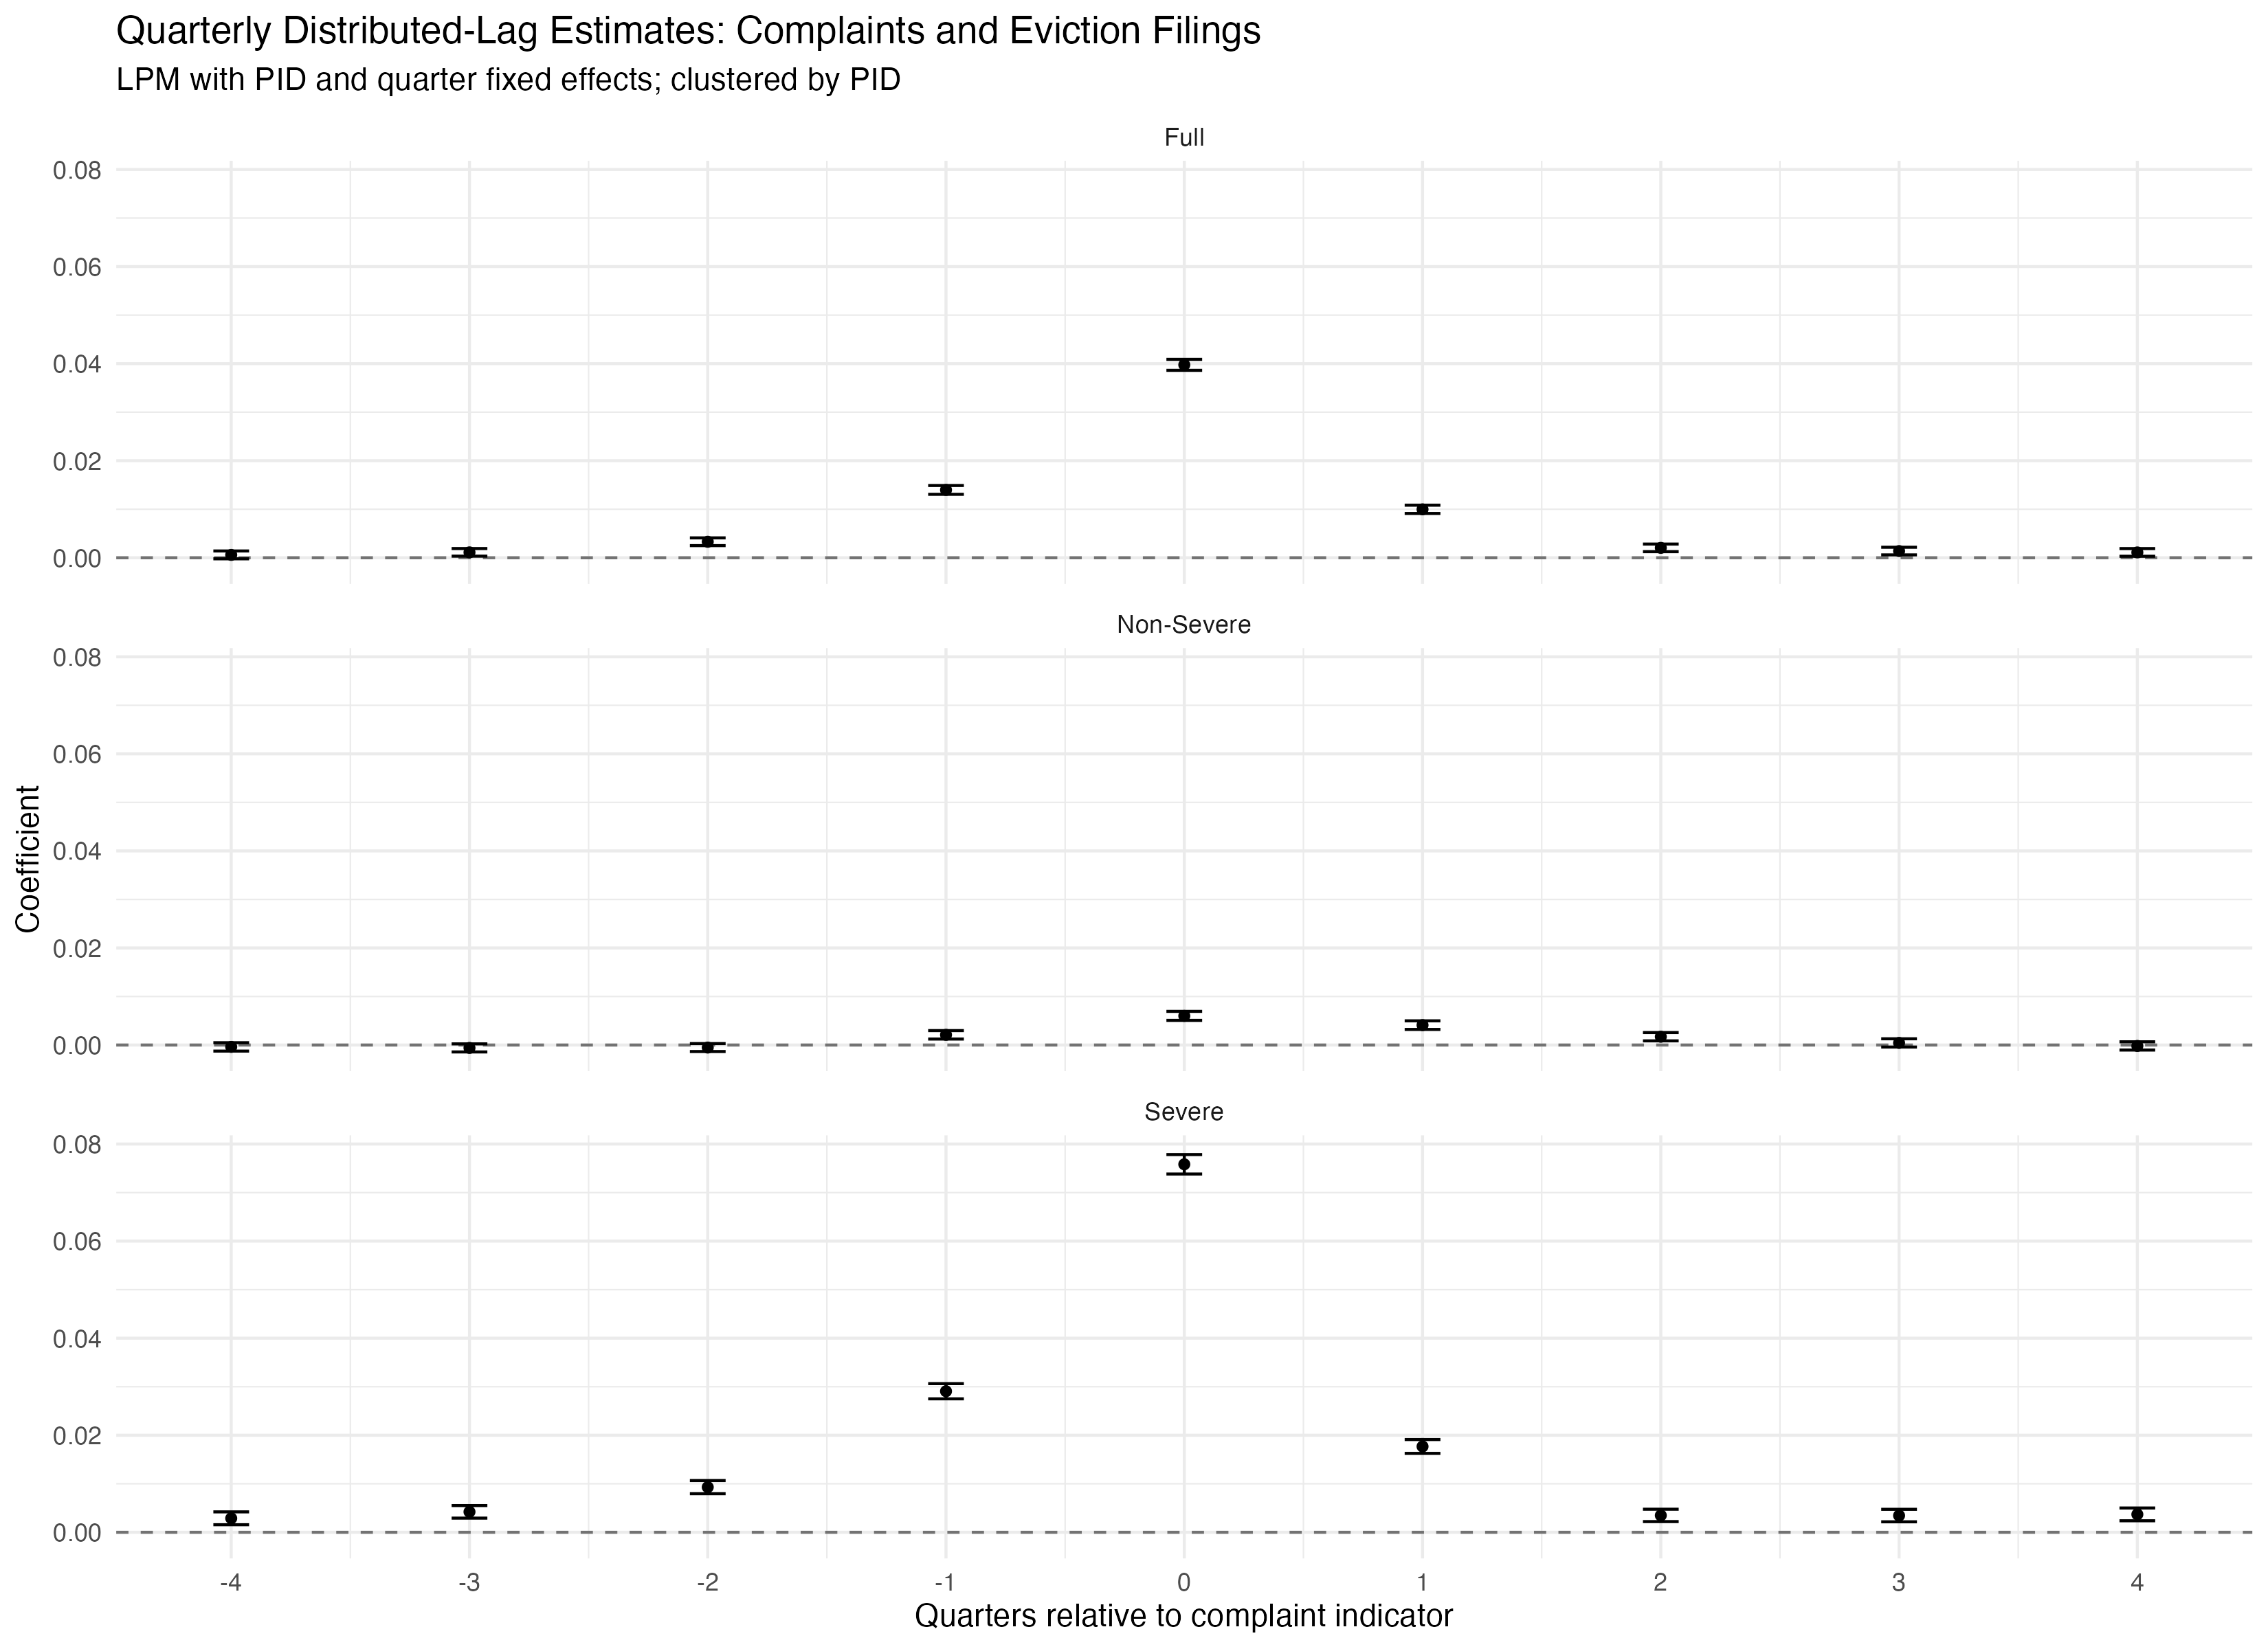
\includegraphics[width=1\linewidth,height=\textheight,keepaspectratio]{../output/retaliatory-evictions/figs/retaliatory_quarterly_distlag_coefficients.png}

}

\caption{Distributed-lag coefficients (pre-COVID): effect of complaint
indicators at lag/lead k on eviction filing indicator. Panels are
labeled Full, Non-Severe, and Severe. PID and period FE; SE clustered by
PID.}

\end{figure}%

\section{\texorpdfstring{\texttt{\%\ Black} Heterogeneity in Distributed
Lags}{\% Black Heterogeneity in Distributed Lags}}\label{black-heterogeneity-in-distributed-lags}

\begin{figure}[H]

{\centering 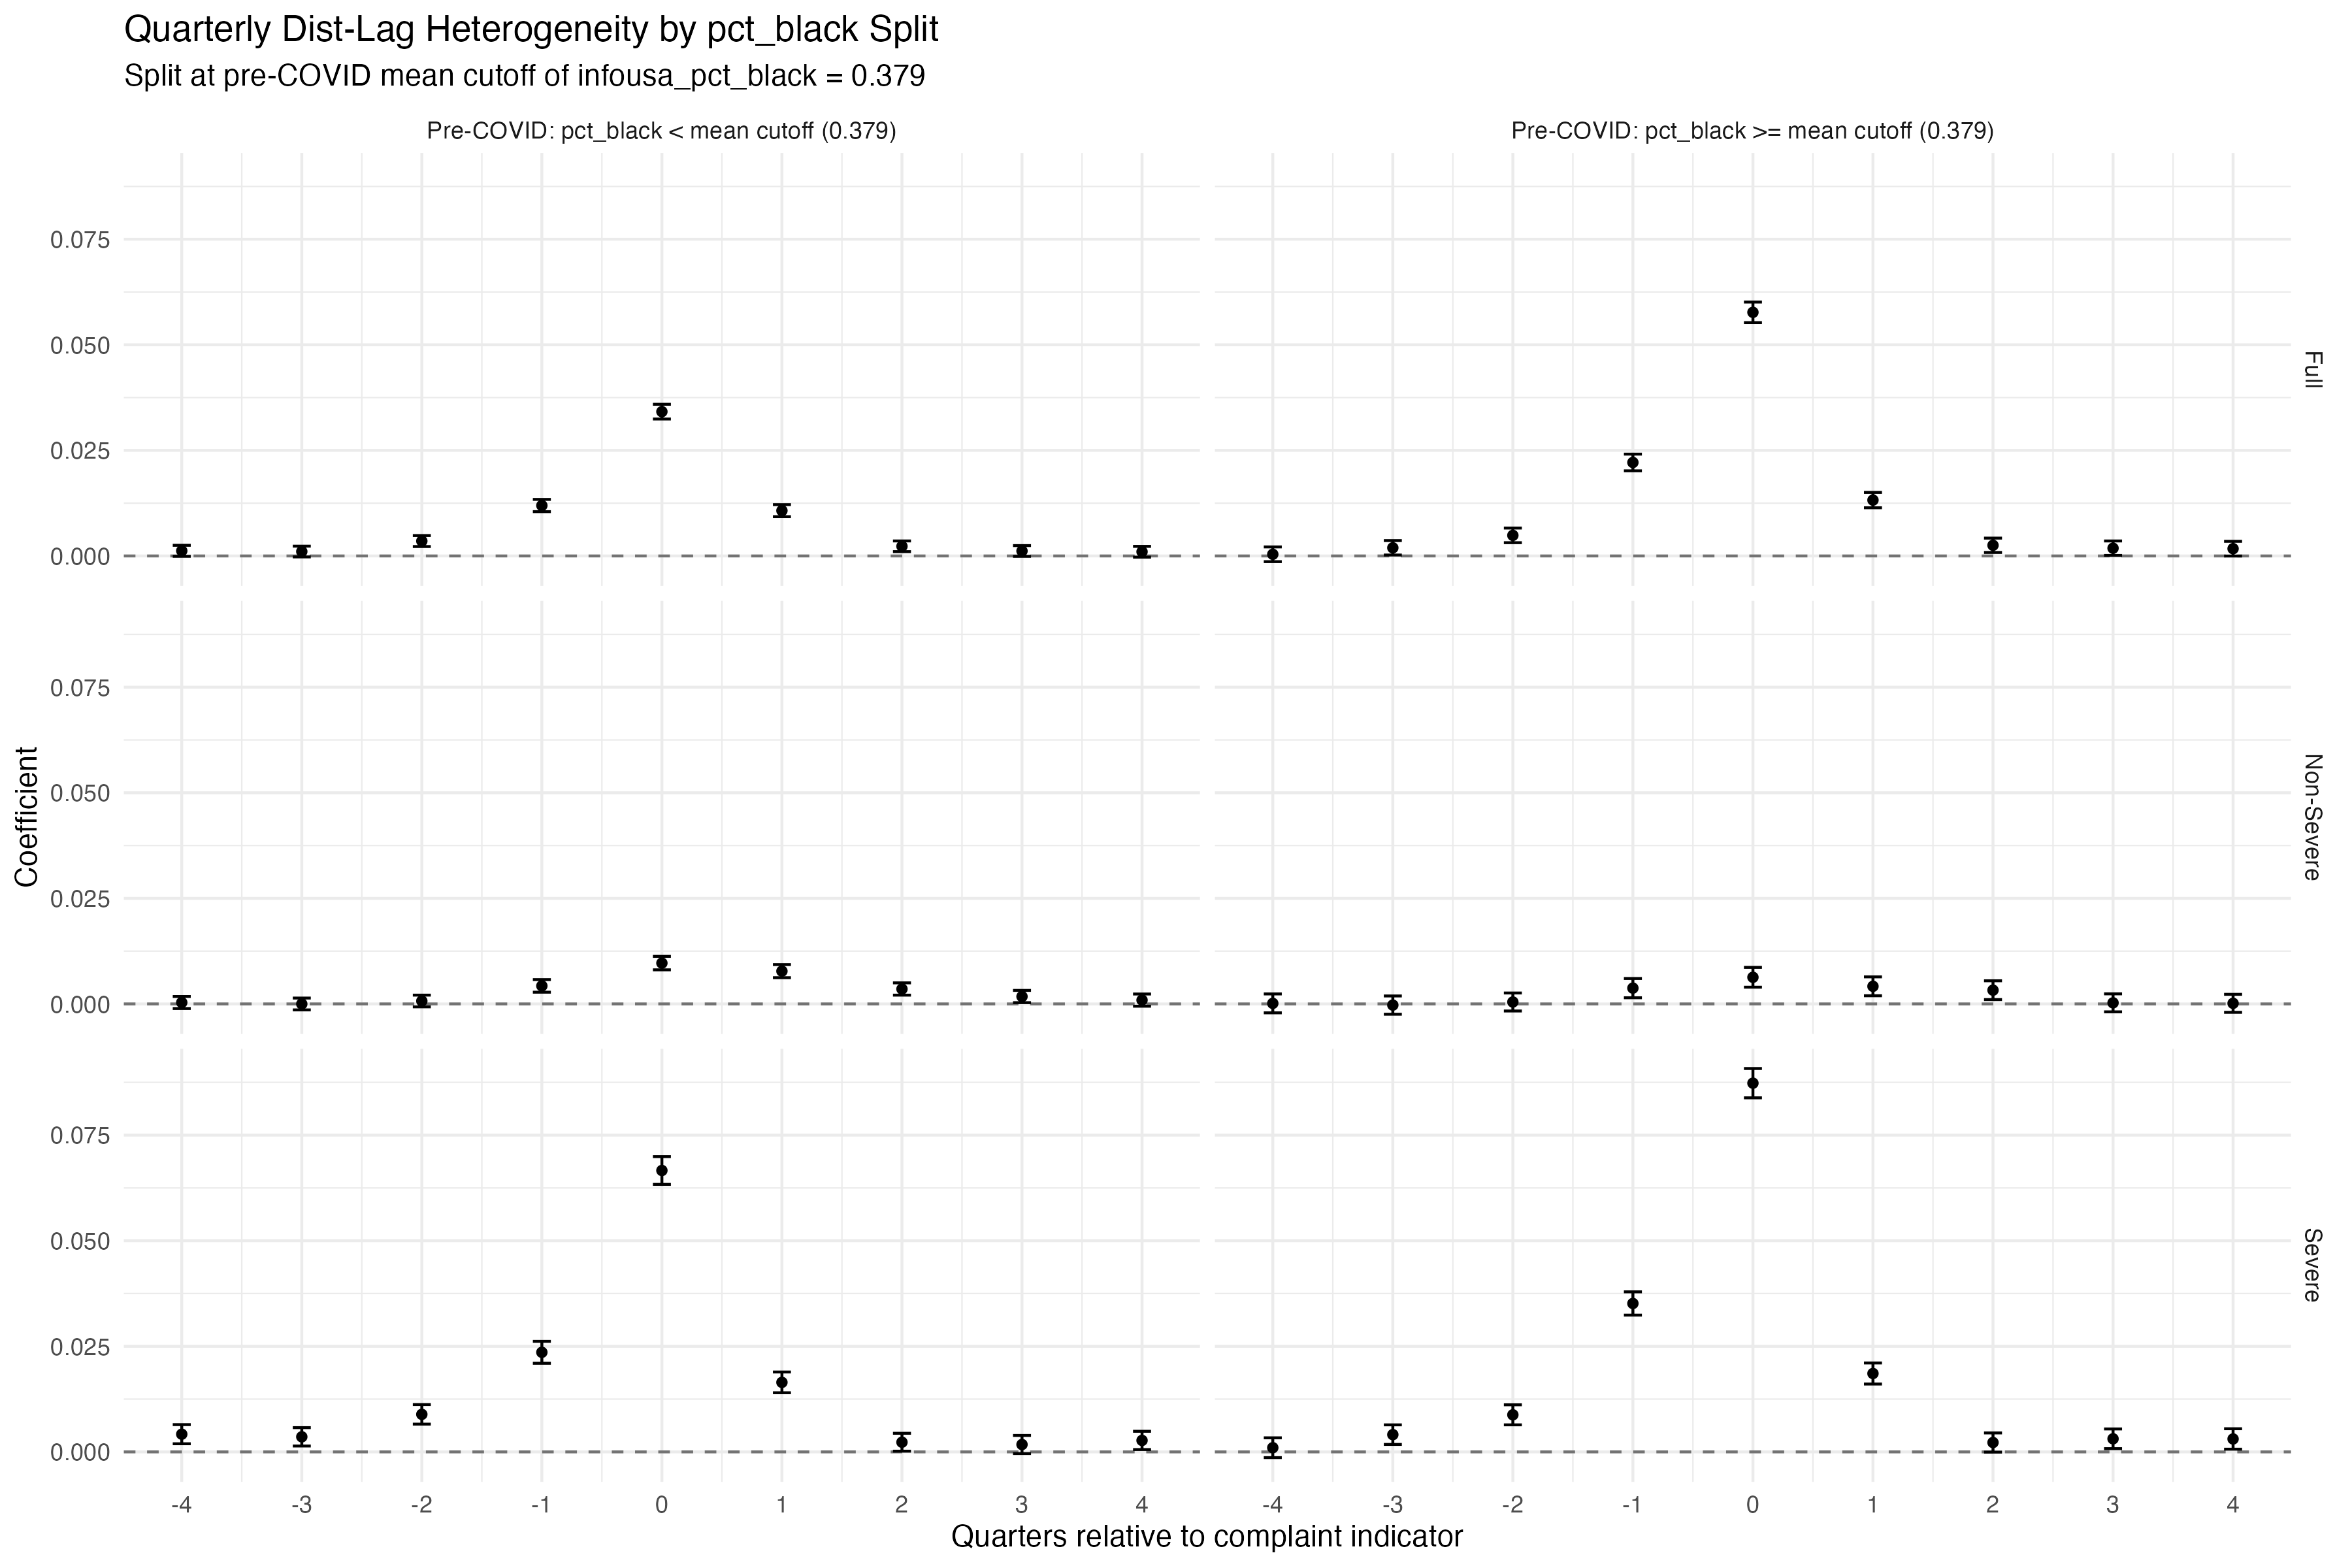
\includegraphics[width=1\linewidth,height=\textheight,keepaspectratio]{../output/retaliatory-evictions/figs/retaliatory_quarterly_distlag_coefficients_black_split.png}

}

\caption{Distributed-lag coefficients by high/low pct black split
(cutoff from pre-COVID distribution rule configured in script).}

\end{figure}%

\section{One-Month Back-Rent
Regressions}\label{one-month-back-rent-regressions}

Case assignment for this block:

\begin{itemize}
\tightlist
\item
  Outcome: \texttt{one\_month\_back\_rent\ =\ 1} when
  \texttt{total\_rent\ /\ ongoing\_rent} is within \texttt{1\ ±\ tol}
  (default \texttt{tol\ =\ 0.10}).
\item
  \texttt{retaliatory\_severe\ =\ 1} if an eviction case's PID-period
  has a severe complaint in the same period or within
  \texttt{±\ bandwidth} periods (default bandwidth is \texttt{2}
  quarters).
\item
  \texttt{high\_black\_split\ =\ 1} if building
  \texttt{infousa\_pct\_black} is above the pre-COVID mean cutoff.
\item
  Defendant race category from case-level imputation
  (\texttt{r/impute-race.R} output): \texttt{black} if
  \texttt{case\_p\_black\ \textgreater{}=\ 0.8}, \texttt{white} if
  \texttt{case\_p\_white\ \textgreater{}=\ 0.8}, and \texttt{unknown}
  otherwise.
\item
  In the defendant-race interaction model, \texttt{white} is the
  reference category.
\end{itemize}

\begin{table}[!h]
\centering
\caption{\label{tab:one-month-retaliatory-status}Pre-COVID case assignment by severe-complaint proximity}
\centering
\fontsize{8}{10}\selectfont
\begin{tabular}[t]{lrl}
\toprule
Status & Cases & Share\\
\midrule
\cellcolor{gray!10}{non\_retaliatory} & \cellcolor{gray!10}{86770} & \cellcolor{gray!10}{61.7\%}\\
same\_period\_severe & 25554 & 18.2\%\\
\cellcolor{gray!10}{within\_bw\_severe\_not\_same\_period} & \cellcolor{gray!10}{28341} & \cellcolor{gray!10}{20.1\%}\\
\bottomrule
\end{tabular}
\end{table}

\begin{table}[!h]
\centering
\caption{\label{tab:one-month-retaliatory-sample}Regression sample summary (pre-COVID; PID + year FE specs)}
\centering
\resizebox{\ifdim\width>\linewidth\linewidth\else\width\fi}{!}{
\fontsize{8}{10}\selectfont
\begin{tabular}[t]{lrrlllllll}
\toprule
Spec & N & Mean(1 month rent) & Same-period severe share & Within-bw severe (not same period) share & Above-mean pct black share & Defendant race: Black & Defendant race: White & Defendant race: Unknown & Defendant race impute-ok share\\
\midrule
\cellcolor{gray!10}{Status dummies only} & \cellcolor{gray!10}{115107} & \cellcolor{gray!10}{0.1898} & \cellcolor{gray!10}{18.2\%} & \cellcolor{gray!10}{20.1\%} & \cellcolor{gray!10}{55.6\%} & \cellcolor{gray!10}{--} & \cellcolor{gray!10}{--} & \cellcolor{gray!10}{--} & \cellcolor{gray!10}{99.5\%}\\
Status x building above-mean pct black & 90737 & 0.1885 & 18.4\% & 21.3\% & 55.6\% & -- & -- & -- & 99.5\%\\
\bottomrule
\end{tabular}}
\end{table}

\begin{center}
\resizebox{\linewidth}{!}{%
\begin{tabular}{lcc}
   \tabularnewline \midrule \midrule
   Dependent Variable: & \multicolumn{2}{c}{one\_month\_back\_rent}\\
   Model:                                                      & (1)                    & (2)\\  
   \midrule
   \emph{Variables}\\
   Same-period severe                                          & 0.017$^{***}$          & -0.011\\   
                                                               & (0.006)                & (0.012)\\   
   One-quarter pre/post severe                                 & $-5.95\times 10^{-5}$  & -0.019$^{*}$\\   
                                                               & (0.006)                & (0.010)\\   
   Above-mean building pct black                               &                        & -0.0003\\   
                                                               &                        & (0.010)\\   
   Same-period severe x above-mean building pct black          &                        & 0.046$^{***}$\\   
                                                               &                        & (0.016)\\   
   One-quarter pre/post severe x above-mean building pct black &                        & 0.032$^{**}$\\   
                                                               &                        & (0.013)\\   
   \% cases filed in quarter of complaint                      & 18.2                   & 18.4\\  
   \% cases in one-quarter pre/post window                     & 20.1                   & 21.3\\  
   \midrule
   \emph{Fixed-effects}\\
   PID                                                         & Yes                    & Yes\\  
   year                                                        & Yes                    & Yes\\  
   \midrule
   \emph{Fit statistics}\\
   Observations                                                & 115,107                & 90,737\\  
   R$^2$                                                       & 0.29134                & 0.29007\\  
   Within R$^2$                                                & 0.00025                & 0.00063\\  
   \midrule \midrule
   \multicolumn{3}{l}{\emph{Clustered (PID) standard-errors in parentheses}}\\
   \multicolumn{3}{l}{\emph{Signif. Codes: ***: 0.01, **: 0.05, *: 0.1}}\\
\end{tabular}
}
\end{center}

\subsection{Poisson (PPML) Regressions: Months Back
Rent}\label{poisson-ppml-regressions-months-back-rent}

The same three specifications are repeated using Poisson (PPML) with
\texttt{months\_back\_rent} (= \texttt{total\_rent\ /\ ongoing\_rent},
continuous) as the outcome. Coefficients are log-multiplicative; SEs
clustered by PID.

\begin{center}
\resizebox{\linewidth}{!}{%
\begin{tabular}{lcc}
   \tabularnewline \midrule \midrule
   Dependent Variable: & \multicolumn{2}{c}{months\_back\_rent}\\
   Model:                                                      & (1)           & (2)\\  
   \midrule
   \emph{Variables}\\
   Same-period severe                                          & -0.027$^{**}$ & 0.025\\   
                                                               & (0.013)       & (0.026)\\   
   One-quarter pre/post severe                                 & 0.005         & 0.028\\   
                                                               & (0.010)       & (0.017)\\   
   Above-mean building pct black                               &               & 0.017\\   
                                                               &               & (0.023)\\   
   Same-period severe x above-mean building pct black          &               & -0.080$^{**}$\\   
                                                               &               & (0.031)\\   
   One-quarter pre/post severe x above-mean building pct black &               & -0.047$^{**}$\\   
                                                               &               & (0.022)\\   
   \% cases filed in quarter of complaint                      & 18.2          & 18.4\\  
   \% cases in one-quarter pre/post window                     & 20.1          & 21.3\\  
   \midrule
   \emph{Fixed-effects}\\
   PID                                                         & Yes           & Yes\\  
   year                                                        & Yes           & Yes\\  
   \midrule
   \emph{Fit statistics}\\
   Observations                                                & 115,043       & 90,679\\  
   Squared Correlation                                         & 0.48646       & 0.49284\\  
   Pseudo R$^2$                                                & 0.16481       & 0.16303\\  
   BIC                                                         & 605,399.7     & 465,151.8\\  
   \midrule \midrule
   \multicolumn{3}{l}{\emph{Clustered (PID) standard-errors in parentheses}}\\
   \multicolumn{3}{l}{\emph{Signif. Codes: ***: 0.01, **: 0.05, *: 0.1}}\\
\end{tabular}
}
\end{center}

\subsection{OLS Log-Rent Regression: log(Total Rent) \textbar{}
log(Ongoing
Rent)}\label{ols-log-rent-regression-logtotal-rent-logongoing-rent}

Outcome is \texttt{log(total\_rent)} with \texttt{log(ongoing\_rent)}
entered as a continuous covariate. Conditioning on log ongoing rent
removes the mechanical correlation between total back rent and rent
level across tenants. The coefficient on \texttt{retaliatory\_status}
therefore captures the percentage difference in total back rent
\emph{claimed} for retaliatory versus non-retaliatory cases, holding the
monthly rent fixed. A negative coefficient means landlords file for less
back rent in retaliatory cases --- i.e., the filing is not primarily
about recovering arrears.

\begin{center}
\resizebox{\linewidth}{!}{%
\begin{tabular}{lcc}
   \tabularnewline \midrule \midrule
   Dependent Variable: & \multicolumn{2}{c}{log(total\_rent)}\\
   Model:                                                      & (1)           & (2)\\  
   \midrule
   \emph{Variables}\\
   Same-period severe                                          & -0.025$^{**}$ & 0.018\\   
                                                               & (0.012)       & (0.024)\\   
   One-quarter pre/post severe                                 & 0.005         & 0.029$^{*}$\\   
                                                               & (0.008)       & (0.015)\\   
   log(ongoing\_rent)                                          & 0.693$^{***}$ & 0.695$^{***}$\\   
                                                               & (0.019)       & (0.021)\\   
   Above-mean building pct black                               &               & -0.001\\   
                                                               &               & (0.017)\\   
   Same-period severe x above-mean building pct black          &               & -0.068$^{**}$\\   
                                                               &               & (0.028)\\   
   One-quarter pre/post severe x above-mean building pct black &               & -0.051$^{***}$\\   
                                                               &               & (0.019)\\   
   \% cases filed in quarter of complaint                      & 18.2          & 18.4\\  
   \% cases in one-quarter pre/post window                     & 20.1          & 21.3\\  
   \midrule
   \emph{Fixed-effects}\\
   PID                                                         & Yes           & Yes\\  
   year                                                        & Yes           & Yes\\  
   \midrule
   \emph{Fit statistics}\\
   Observations                                                & 112,729       & 88,859\\  
   R$^2$                                                       & 0.49715       & 0.50065\\  
   Within R$^2$                                                & 0.04103       & 0.04208\\  
   \midrule \midrule
   \multicolumn{3}{l}{\emph{Clustered (PID) standard-errors in parentheses}}\\
   \multicolumn{3}{l}{\emph{Signif. Codes: ***: 0.01, **: 0.05, *: 0.1}}\\
\end{tabular}
}
\end{center}

\section{Equilibrium Maintenance
Analysis}\label{equilibrium-maintenance-analysis}

This section examines whether landlords adjust maintenance investment
(proxied by permit activity) in response to eviction pressure and tenant
composition, and whether permit activity responds dynamically to severe
complaints.

\subsection{Baseline Maintenance Permit
Regressions}\label{baseline-maintenance-permit-regressions}

Poisson (PPML) regressions of \texttt{total\_permits} on building-level
eviction filing intensity and racial composition, with
\texttt{log(total\_units)} as offset. Main specifications use EB
pre-COVID filing intensity (\texttt{filing\_rate\_eb\_pre\_covid}) with:

\begin{itemize}
\tightlist
\item
  a high-filing dummy (\texttt{\textgreater{}=\ 15\%})
\item
  filing bins: \texttt{{[}0,1)}, \texttt{{[}1,5)}, \texttt{{[}5,10)},
  \texttt{{[}10,20)}, \texttt{{[}20,inf)} (all on EB rates)
\end{itemize}

The rent-augmented variants add mean inflation-adjusted log rent (within
PID over 2011--2019) to partial out rent-driven maintenance incentives.

\begin{center}
\resizebox{\linewidth}{!}{%
\begin{tabular}{lcccc}
   \tabularnewline \midrule \midrule
   Dependent Variable: & \multicolumn{4}{c}{total\_permits}\\
   Model:                                    & (1)            & (2)            & (3)            & (4)\\  
   \midrule
   \emph{Variables}\\
   above\_mean\_pct\_black\_btTRUE           & -0.375$^{***}$ & -0.327$^{***}$ & -0.379$^{***}$ & -0.335$^{***}$\\   
                                             & (0.007)        & (0.009)        & (0.007)        & (0.009)\\   
   high\_filing\_eb                          & -0.153$^{***}$ & -0.101$^{***}$ &                &   \\   
                                             & (0.012)        & (0.012)        &                &   \\   
   mean\_log\_med\_rent\_inf\_adj\_PID       &                & 0.376$^{***}$  &                & 0.383$^{***}$\\   
                                             &                & (0.010)        &                & (0.010)\\   
   filing\_bin\_eb $=$ [1,5)")               &                &                & 0.093$^{***}$  & -0.003\\   
                                             &                &                & (0.008)        & (0.010)\\   
   filing\_bin\_eb $=$ [5,10)")              &                &                & -0.154$^{***}$ & -0.130$^{***}$\\   
                                             &                &                & (0.009)        & (0.011)\\   
   filing\_bin\_eb $=$ [10,20)")             &                &                & -0.130$^{***}$ & -0.090$^{***}$\\   
                                             &                &                & (0.011)        & (0.012)\\   
   filing\_bin\_eb $=$ [20,inf)")            &                &                & -0.219$^{***}$ & -0.179$^{***}$\\   
                                             &                &                & (0.015)        & (0.016)\\   
   \midrule
   \emph{Fixed-effects}\\
   building\_type                            & Yes            & Yes            & Yes            & Yes\\  
   year                                      & Yes            & Yes            & Yes            & Yes\\  
   quality\_grade                            & Yes            & Yes            & Yes            & Yes\\  
   year\_blt\_decade                         & Yes            & Yes            & Yes            & Yes\\  
   num\_units\_bin                           & Yes            & Yes            & Yes            & Yes\\  
   GEOID                                     & Yes            & Yes            & Yes            & Yes\\  
   has\_rent\_data                           & Yes            &                & Yes            & \\  
   \midrule
   \emph{Fit statistics}\\
   Observations                              & 1,703,026      & 750,270        & 1,683,789      & 743,824\\  
   Squared Correlation                       & 0.31379        & 0.25057        & 0.32030        & 0.25933\\  
   Pseudo R$^2$                              & 0.20782        & 0.26005        & 0.20954        & 0.26192\\  
   BIC                                       & 1,144,296.2    & 615,091.5      & 1,121,025.3    & 602,300.0\\  
   \midrule \midrule
   \multicolumn{5}{l}{\emph{IID standard-errors in parentheses}}\\
   \multicolumn{5}{l}{\emph{Signif. Codes: ***: 0.01, **: 0.05, *: 0.1}}\\
\end{tabular}
}
\end{center}

\subsection{Landlord Response to Severe
Complaints}\label{landlord-response-to-severe-complaints}

The following coefplot shows estimates from a PPML regression of
\texttt{total\_permits} on contemporaneous, lagged (past quarters), and
lead (future quarters) severe complaint counts, with PID and year fixed
effects. Lead terms serve as pre-trend checks.

\begin{figure}[H]

{\centering 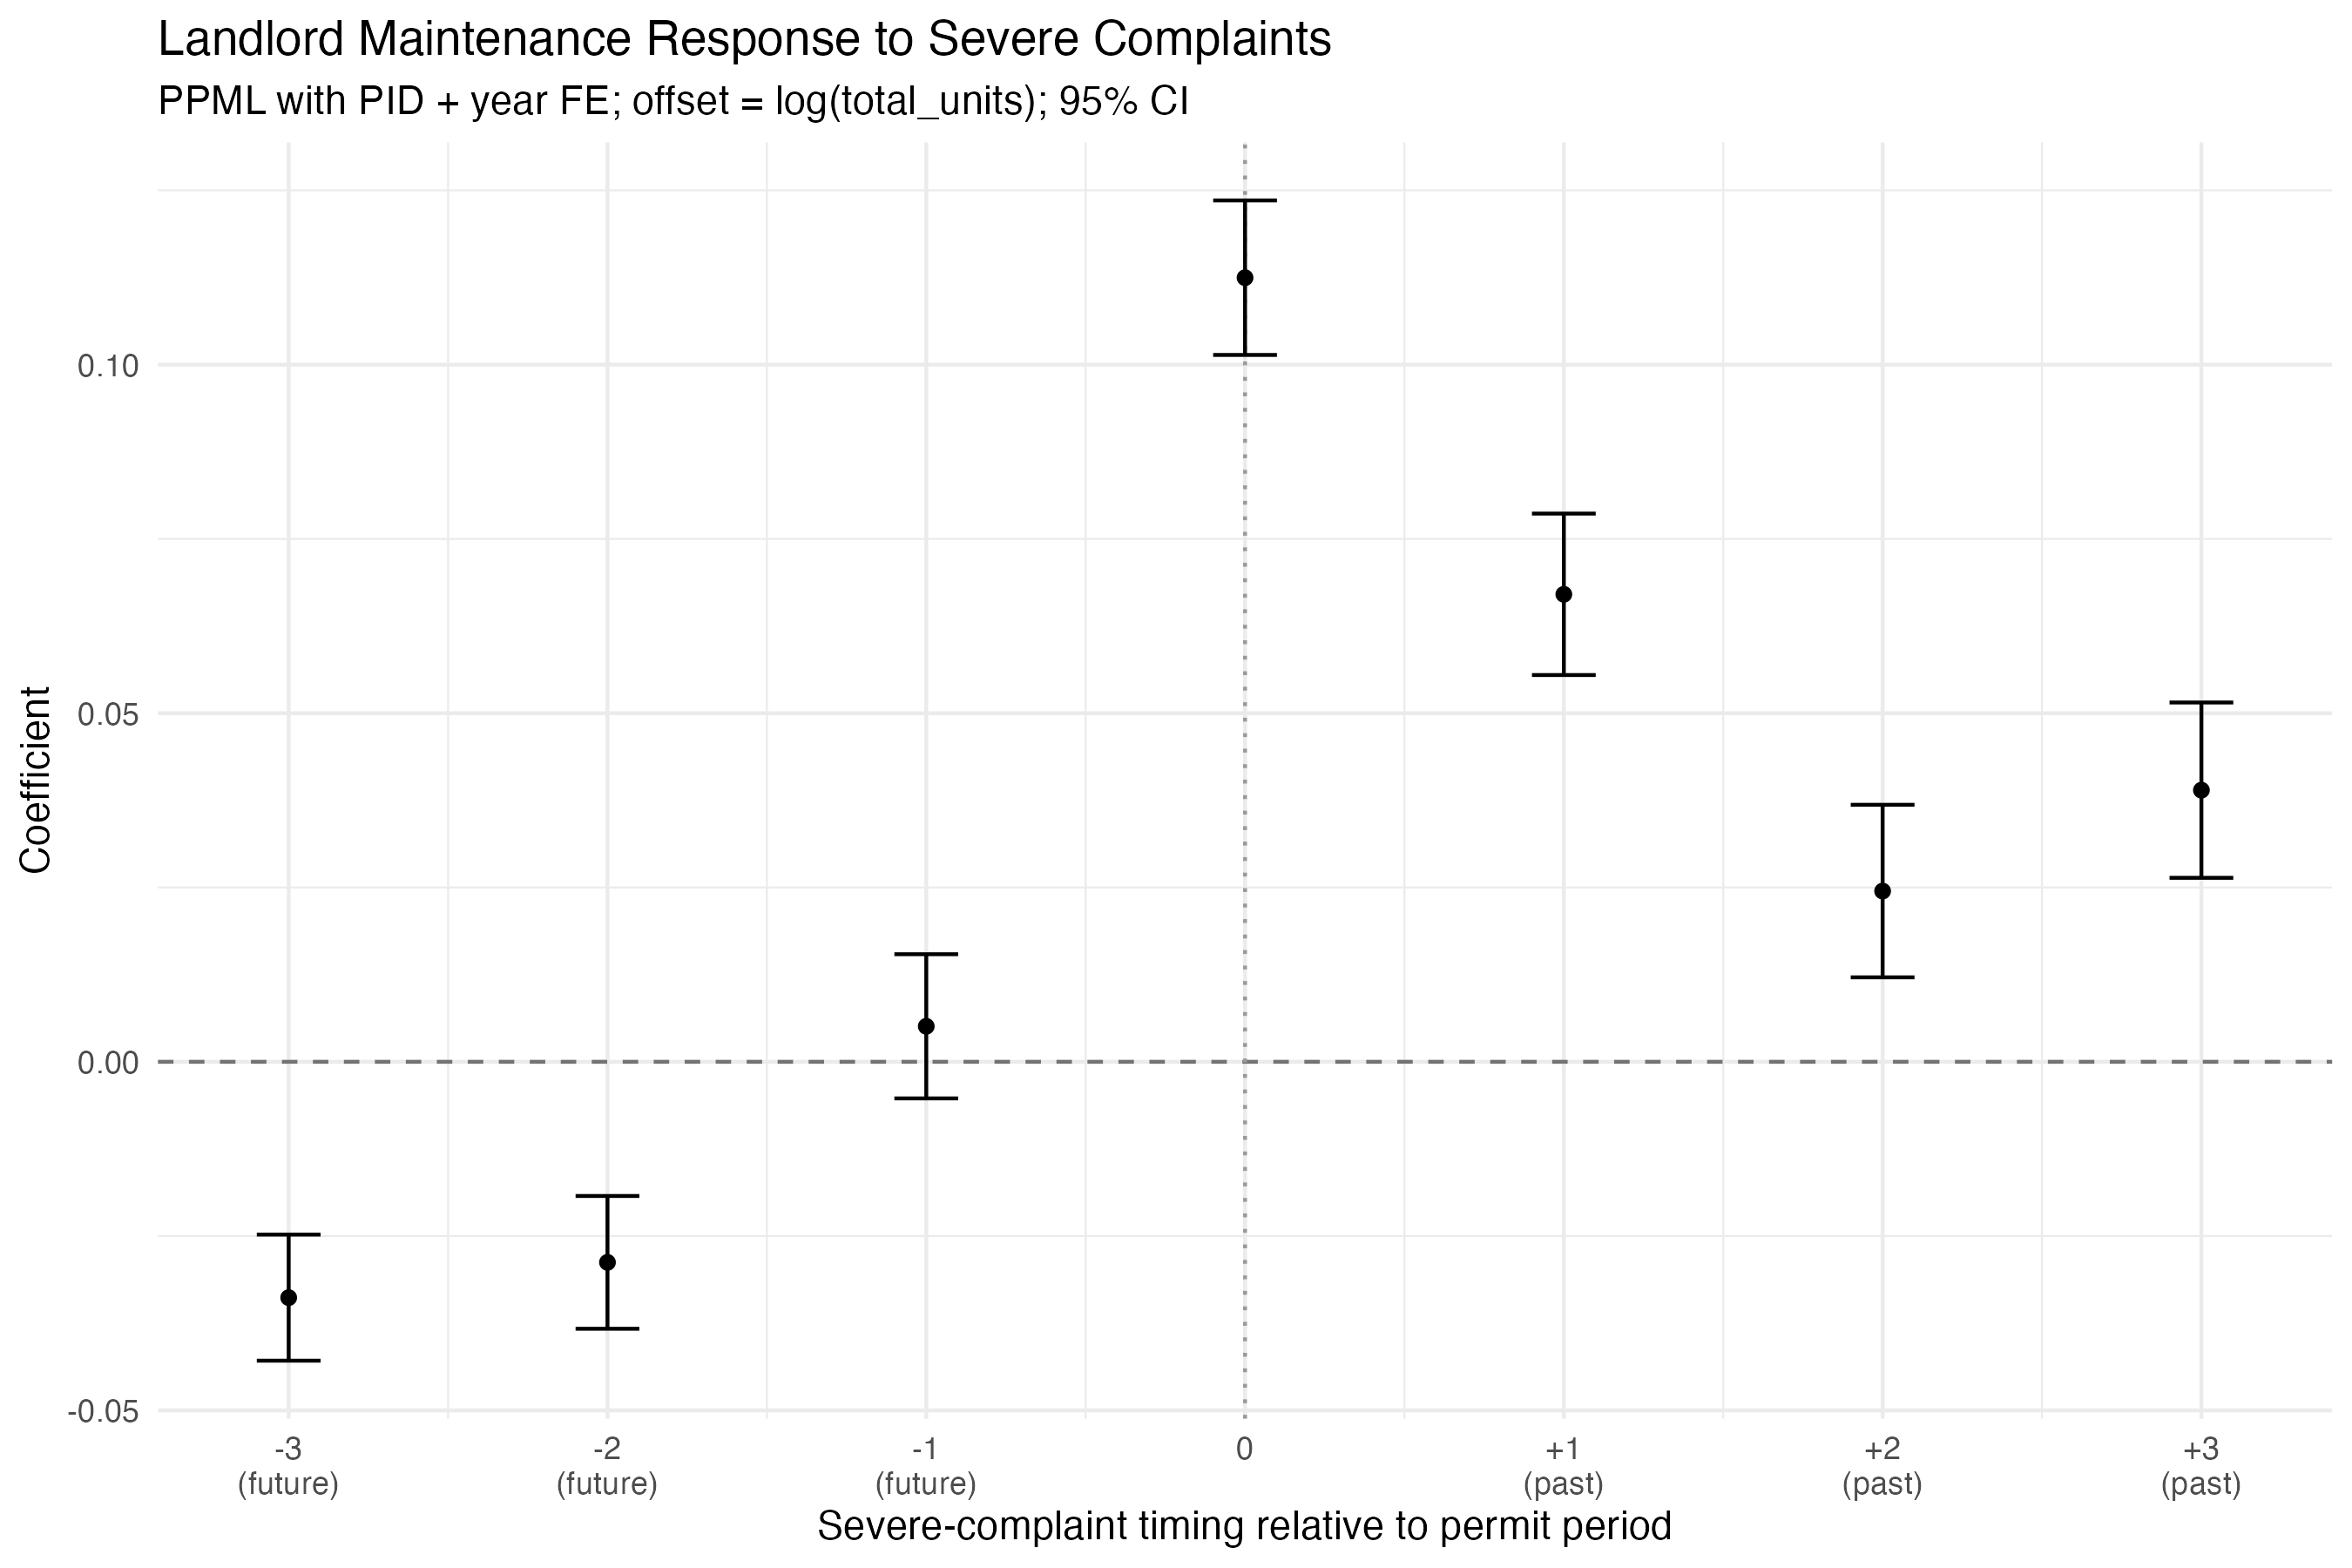
\includegraphics[width=1\linewidth,height=\textheight,keepaspectratio]{../output/retaliatory-evictions/figs/retaliatory_quarterly_landlord_response_plot.png}

}

\caption{Landlord maintenance response to severe complaints: PPML
event-study. Negative timing = complaints occur in future periods
relative to permit outcome (pre-trend check); positive timing = past
complaints. PID + year FE; offset = log(total\_units); 95\% CI.}

\end{figure}%

\section{Notes}\label{notes}

\begin{itemize}
\tightlist
\item
  Raw long-run filing-rate maintenance regressions are moved to the
  appendix section below.
\item
  This writeup intentionally excludes same-period, targeting, LP-DiD,
  and complaint-suppression blocks.
\item
  For complaint-suppression specifications and interpretation, use
  \texttt{writeups/comp-statics-annual-race.qmd}.
\end{itemize}

\section{Appendix: Raw Filing
Robustness}\label{appendix-raw-filing-robustness}

These regressions mirror the baseline maintenance models but replace EB
filing intensity with raw long-run pre-2019 filing rate (same 15\%
high-filing cutoff and same bins), for robustness only.

\begin{center}
\resizebox{\linewidth}{!}{%
\begin{tabular}{lcccc}
   \tabularnewline \midrule \midrule
   Dependent Variable: & \multicolumn{4}{c}{total\_permits}\\
   Model:                                    & (1)            & (2)            & (3)            & (4)\\  
   \midrule
   \emph{Variables}\\
   above\_mean\_pct\_black\_btTRUE           & -0.373$^{***}$ & -0.326$^{***}$ & -0.362$^{***}$ & -0.316$^{***}$\\   
                                             & (0.007)        & (0.009)        & (0.007)        & (0.009)\\   
   high\_filing\_raw                         & -0.211$^{***}$ & -0.137$^{***}$ &                &   \\   
                                             & (0.013)        & (0.014)        &                &   \\   
   mean\_log\_med\_rent\_inf\_adj\_PID       &                & 0.375$^{***}$  &                & 0.352$^{***}$\\   
                                             &                & (0.010)        &                & (0.010)\\   
   filing\_bin\_raw $=$ [1,5)")              &                &                & -0.150$^{***}$ & -0.184$^{***}$\\   
                                             &                &                & (0.010)        & (0.011)\\   
   filing\_bin\_raw $=$ [5,10)")             &                &                & -0.197$^{***}$ & -0.137$^{***}$\\   
                                             &                &                & (0.009)        & (0.011)\\   
   filing\_bin\_raw $=$ [10,20)")            &                &                & -0.217$^{***}$ & -0.151$^{***}$\\   
                                             &                &                & (0.013)        & (0.014)\\   
   filing\_bin\_raw $=$ [20,inf)")           &                &                & -0.324$^{***}$ & -0.232$^{***}$\\   
                                             &                &                & (0.015)        & (0.016)\\   
   \midrule
   \emph{Fixed-effects}\\
   building\_type                            & Yes            & Yes            & Yes            & Yes\\  
   year                                      & Yes            & Yes            & Yes            & Yes\\  
   quality\_grade                            & Yes            & Yes            & Yes            & Yes\\  
   year\_blt\_decade                         & Yes            & Yes            & Yes            & Yes\\  
   num\_units\_bin                           & Yes            & Yes            & Yes            & Yes\\  
   GEOID                                     & Yes            & Yes            & Yes            & Yes\\  
   has\_rent\_data                           & Yes            &                & Yes            & \\  
   \midrule
   \emph{Fit statistics}\\
   Observations                              & 1,703,026      & 750,270        & 1,703,026      & 750,270\\  
   Squared Correlation                       & 0.31361        & 0.25042        & 0.31484        & 0.25360\\  
   Pseudo R$^2$                              & 0.20788        & 0.26008        & 0.20841        & 0.26058\\  
   BIC                                       & 1,144,210.6    & 615,062.0      & 1,143,500.9    & 614,705.9\\  
   \midrule \midrule
   \multicolumn{5}{l}{\emph{IID standard-errors in parentheses}}\\
   \multicolumn{5}{l}{\emph{Signif. Codes: ***: 0.01, **: 0.05, *: 0.1}}\\
\end{tabular}
}
\end{center}




\end{document}
